\documentclass[a4paper]{article}

\usepackage[english]{babel}
\usepackage[utf8]{inputenc}
\usepackage{amsmath}
\usepackage{graphicx}
\usepackage[colorinlistoftodos]{todonotes}

\usepackage{theorem}
\usepackage{amssymb}

\usepackage{hyperref}

\usepackage{caption}
\usepackage{subcaption}

\newenvironment{proof}{{\bf Proof:  }}{\hfill\rule{2mm}{2mm}}

\newtheorem{fact}{Fact}[section]
\newtheorem{lemma}[fact]{Lemma}
\newtheorem{theorem}[fact]{Theorem}
\newtheorem{definition}[fact]{Definition}
\newtheorem{corollary}[fact]{Corollary}
\newtheorem{proposition}[fact]{Proposition}
\newtheorem{claim}[fact]{Claim}
\newtheorem{exercise}[fact]{Exercise}

\usepackage{algorithm}
\usepackage{algorithmic}

\makeatletter
\newcommand{\distas}[1]{\mathbin{\overset{#1}{\kern\z@\sim}}}%
\newsavebox{\mybox}\newsavebox{\mysim}
\newcommand{\distras}[1]{%
  \savebox{\mybox}{\hbox{\kern3pt$\scriptstyle#1$\kern3pt}}%
  \savebox{\mysim}{\hbox{$\sim$}}%
  \mathbin{\overset{#1}{\kern\z@\resizebox{\wd\mybox}{\ht\mysim}{$\sim$}}}%
}
\makeatother

\newcommand{\RT}[1]{\marginpar{\footnotesize\color{red}RT: #1}}

\title{Law of Large Graphs}

\date{\today}

\begin{document}
\maketitle

\section{Introduction}

Mean is one of the most important and basic concept in statistics. Motivated by the law of large numbers, sample mean is always considered to be the best estimate of the population mean. Nowadays we take averages almost everywhere, from the fundamental elements in Euclidean space to more general objects, like shapes, documents and graphs.

However, contradict to the general intuition, arithmetic average should not be our first choice all the time. In 1955, Stein's paradox \cite{efron1977stein} shows the inadmissibility of the sample mean when there are more than three normal distributions. The fact that James-Stein estimator dominates the sample mean makes it less preferable to take the average in that situation. 27 years later, Gutmann proved that this cannot occur when the sample spaces are finite \cite{gutmann1982stein}. But even when sample mean is admissible, it doesn't close the door of other estimators to be better in some cases. So in a specific situation, for instance a collection of graphs considered in this paper, there is always a chance to have a better estimator compared to the sample mean.

Before introducing the new estimator other than the sample mean for graphs, we need to know what the mean of a collection of graphs is. Although it can be defined in various ways, we pick the natural definition as the proportions of the existence of an edge between any pair of vertices. Estimating the mean of a population of graphs based on a sample is becoming more and more important both in statistical inference and in various applications like connectomics, social networks, etc.

Element-wise maximum likelihood estimate (MLE), which happens to be the sample mean in many situations, is a reasonable estimator if we only consider the independent edge model (IEM) \cite{bollobas2007phase} without taking any graph structure into account. However, it does not perform very well especially when only a few observations are available, which happens a lot in practice.

Intuitively, an estimator incorporating the graph structure is preferable than the entry-wise MLE. But we don't have any knowledge about the structure of the graphs in general. So it is hard to take advantage of the unknown graph structure.

One of the most important structures is the community structure in which vertices are clustered into different communities and the ones of the same community behave similarly. The stochastic blockmodel (SBM) \cite{holland1983stochastic} captures such structural property and is widely used in modeling networks.

Meanwhile, the latent positions model (LPM) \cite{hoff2002latent}, a much more general model compared to SBM, proposes a way to parameterize the graph structure by latent positions associated with each vertex. The random dot product graph (RDPG) \cite{young2007random, nickel2007random} which is a special case of LPM stays in between and motivates our estimator. In this paper, we analyze our estimator in terms of RDPG specifically.

Using the estimates of the latent positions in an RDPG setting based on a truncated eigen-decomposition of the adjacency matrix, we consider a new estimator for the mean of the collection of graphs which captures the low-rank structure. In this study, we prove via theory, simulations and real data analysis that it is better than element-wise MLE.

(Future work) Robust estimation, dimension selection, diagonal augmentation, etc.



\section{Models and Estimators}
This work considers the scenario of having $M$ graphs represented as adjacency matrices, $\{A^{(m)}\}$ ($m = 1, \cdots, M$), each having $N$ vertices with known correspondence. The graphs we consider are undirected and unweighted with no self-loops, i.e. each $A^{(m)}$ is a binary symmetric matrix with zeros along the diagonal. An example application of this arises in the field of connectomics, where functional brain imaging data for each subject can be represented as a graph, with each vertex having a defined anatomical correspondence, and an edge between two regions is defined to exist if correlation in activity between the regions reaches a certain threshold.



\subsection{Independent Edge Model}
The first basic model we consider is the independent edge model (IEM) with parameter $P \in [0,1]^{N\times N}$\cite{bollobas2007phase}, where each edge between vertex $i$ and vertex $j$ exists with probability $P_{ij}$ independently of all other edges. In this case, we aim to estimate the mean, i.e. probability matrix $P$, with our observations of the adjacency matrices $\{A^{(m)}\}$ of $M$ graphs.



\subsection{Estimator $\bar{A}$}
Under the IEM, element-wise sample mean of the adjacency matrices $\bar{A}$ is the MLE as well as the least squared estimate for $P$. It is unbiased with entry-wise variance $\mathrm{Var}(\bar{A}_{ij}) = P_{ij} (1-P_{ij})/M$. Moreover, $\bar{A}$ is the uniformly minimum-variance unbiased estimator (UMVUE), i.e. it has the smallest variance among all unbiased estimators.

However, $\bar{A}$ doesn't exploit any graph structure, and sometimes the performance is not very good especially when $M$ is small. For example, when $M=1$, $\bar{A}$ is exactly the binary graph we observe, which is an inaccurate estimate for an arbitrary $P$.



\subsection{Random Dot Product Graph}
In graphs, the adjacencies always depends on the unobserved properties of the corresponding vertices. For example, in a connectomics setting, the two brain regions with similar (some properties?) will have stronger connections.
The latent positions graph model (LPG) proposed by Hoff et. al. (2002) \cite{hoff2002latent} captures such structure. where each vertex is associated with a latent positions that influences the adjacencies for that vertex.
In this model, each vertex $i$ has an associated latent vector $X_i \in \mathbb{R}^d$ sampled from distribution $\mathcal{F}$. Based on those latent positions, the existence of edges are conditionally independent with probability only depends on the latent vectors of the incident vertices through a link function. Generally $d$ is much smaller than the number of vertices $N$, so it is a much more succinct model compared to IEM.

A specific instance of the LPG that we examine in this work is the random dot product graph model (RDPG) \cite{young2007random, nickel2007random} where the link function is the dot product, i.e. the probability of an edge being present between two nodes is the dot product of their latent vectors.

Formally, let $\mathcal{X} \subset \mathbb{R}^d$ be a set such that $x, y \in \mathcal{X}$ implies $\left \langle  x,y \right \rangle \in [0, 1]$, let $X_i\distas{iid} F$ on $\mathcal{X}$, and write $X = [X_1|\cdots|X_N]^T \in \mathbb{R}^{N \times d}$.
A random graph $G$ with adjacency matrix $A$ is said to be an RDPG if
\[
	P(A|X) = \prod_{i<j} \left \langle X_i, X_j \right \rangle^{A_{ij}} \left( 1 - \left \langle X_i, X_j \right \rangle \right)^{1 - A_{ij}}.
\]
In the RDPG model,each vertex $i$ is associated with a latent position $X_i$. Conditioned on the latent positions $X$, the edges $A_{ij} \distas{iid} \text{Bern}(\left \langle X_i, X_j \right \rangle)$.
Note that the probability matrix is the out product of the latent positions, i.e. $P = X X^T$.
%Note that $\mathrm{rank}(P) = \mathrm{rank}(X)$.




\subsection{Estimator $\hat{P}$ Based on Adjacency Spectral Embedding}

Motivated by the RDPG, we consider a new estimator $\hat{P}$ based on the adjacency spectral embedding (ASE) which enforce a low rank approximation on the entry-wise sample mean $\bar{A}$.

Since the graphs are symmetric, we can get $\hat{U} \hat{S} \hat{U}^T$ as the eigen-decomposition of $\bar{A}$, where $\hat{S}$ is a diagonal matrix with non-increasing entries along the diagonal. Then the $d$-dimensional ASE of $\bar{A}$ is the first $d$ columns of $\hat{U} |\hat{S}|^{1/2}$, denoted by $\hat{X} \in \mathbb{R}^{N \times d}$. The rows of $\hat{X}$ represent the estimated latent vectors for each vertex. 
Based on the low rank approximated RDPG representation of the sample mean matrix constructed by ASE, we define our new estimator as $\hat{P} = \hat{X} \hat{X}^T$.

To get $\hat{P}$, we need to specify what dimension $d$ that ASE uses. There are varies ways dealing with dimension selection. In this paper, we consider Zhu and Ghodsi's elbow selection method \cite{zhu2006automatic} and the universal singular value thresholding (USVT) method \cite{chatterjee2015matrix}. Details are discussed in Section \ref{section:dim_select}.

Moreover, since the graphs are hollow, i.e. with zeros along the diagonal, applying ASE directly will lead to a bias in calculating the eigenvalues. To compensate such bias, we use an iterative method developed by Scheinerman and Tucker \cite{scheinerman2010modeling}. Details are discussed in Section \ref{section:diag_aug}.


\begin{algorithm}[H]
\caption{}
\label{algo:basic}
\begin{algorithmic}[1]
\STATE \textbf{Input:} $A^{(1)}, A^{(2)}, \cdots, A^{(M)}$, each $A^{(m)} \in \{0,1\}^{N \times N}$ is symmetric and hollow, with known vertex correspondence;
\STATE Calculate the sample mean graph $\bar{A} = \frac{1}{M}\sum\limits_{m = 1}^M A^{(m)}$;
\STATE Augmented the diagonal of $\bar{A}$ to get $\bar{A} + D$ (see Section \ref{section:diag_aug});
\STATE Select the dimension $d$ to which we are going to embed $\bar{A} + D$ (see Section \ref{section:dim_select});
\STATE Calculate the eigen-decomposition, $\bar{A} + D = \hat{U} \hat{S} \hat{U}^T$;
\STATE Obtain $d$-dimensional ASE $\hat{X} \in \mathbb{R}^{N \times d}$ by the first $d$ columns of $\hat{U} |\hat{S}|^{1/2}$;
\STATE $\hat{P} = \hat{X} \hat{X}^{T}$ is our estimator.
\end{algorithmic}
\end{algorithm}



In order to take advantage of the underlying low rank structure of the RDPG, we use the adjacency spectral embedding (ASE) studied by Sussman et. al. to enforce a low rank approximation on the entry-wise mean matrix $\bar{A}$, which will decrease the variance without losing much in bias if we embed it into the right dimension.

\subsection{Stochastic Block Model as an Random Dot Product Graph}
One of the most important structures is the community structure in which vertices are clustered into different communities such that vertices of the same community behave similarly. Such structural property is captured by the stochastic blockmodel (SBM) \cite{holland1983stochastic}, where each vertex is assigned to a block and the probability that an edge exists between two vertices depends only on their respective block memberships.

Formally, the SBM is parameterized by the number of blocks $K$ (generally way less than the number of vertices $N$), block probability matrix $B \in [0,1]^{K \times K}$ and block proportion vector $\rho \in (0,1)^K$ with $\sum_{k=1}^K \rho_k = 1$. Let $\tau$ represent the block memberships, then for any $i \in [n]$ and $k \in [K]$, $\tau(i) = k$ means vertex $i$ is assigned to block $k$. And each vertex is assigned independently with probability vector $\rho$, i.e. $P(\tau(i) = k) = \rho_k$. Conditioned on $\tau$, each entry of the adjacency matrix $A_{ij}$ is independently sampled from the Bernoulli distribution with parameter $B_{\tau_i,\tau_j}$.

In order to analyze the estimator $\hat{P}$ motivated by RDPG, we move to another representation of SBM based on RDPG. Consider a positive semi-definite $K$-block SBM with a rank $d (\le K)$ block probability matrix $B$, we can always decompose $B$ into $\nu \nu^T$, where $\nu \in \mathbb{R}^{K \times d}$ and each row $\nu_k$ is the shared latent position for all vertices assigned to block $k$. Let $X \in \mathbb{R}^{N \times d}$ with each row to be $X_i = \nu_{\tau_i}$, then we have
\[
	P(A_{ij} = 1|\tau) = B_{\tau_i, \tau_j} = \nu_{\tau_i}^T \nu_{\tau_j}.
\]
Note that the SBM can be seen as an RDPG with $X_i \distas{iid} \sum_{k=1}^K \rho_k \delta_{\nu_k}$, i.e. all vertices in the same block will have identical latent positions.

To better illustrating what an SBM actually looks like, in Figure \ref{fig:SBM_example} we consider a 5-block SBM and plot the corresponding probability matrix and one adjacency matrix generated from it with 200 vertices. From the figure, we can clearly see the structure of 25 blocks in both the probability matrix and the adjacency matrix as a result of 5 different blocks among vertices.

\begin{figure}
\centering
\begin{subfigure}{.5\textwidth}
  \centering
  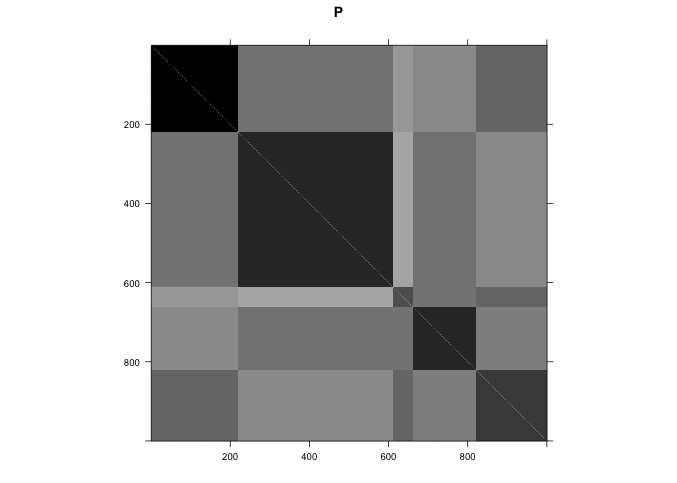
\includegraphics[width=1.2\linewidth]{SBM_P.png}
\end{subfigure}%
\begin{subfigure}{.5\textwidth}
  \centering
  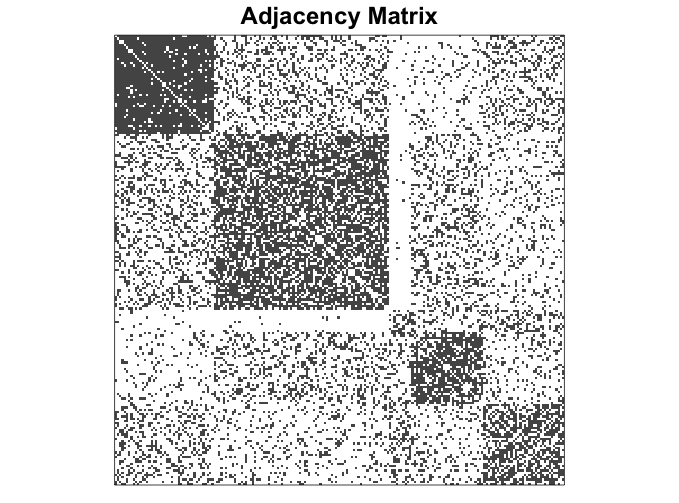
\includegraphics[width=1.2\linewidth]{SBM_A.png}
\end{subfigure}
\caption{Example illustrating the SBM. The figure on the left is the probability matrix $P$ that follows a SBM with $K = 5$ blocks; The other figure shows the adjacency matrix $A$ for 200 vertices generated from the SBM with probability matrix $P$.}
\label{fig:SBM_example}
\end{figure}



\section{Results}

\subsection{Theoretical Results}
\begin{itemize}
\item To compare the performance between $\hat{P}$ and $\bar{A}$, we examine the relative efficiency (RE), in mean squared error (MSE), among the two defined as: $RE_{ij} = \frac{MSE(\hat{P}_{ij})}{MSE(\bar{A}_{ij})}$.
\item
\begin{theorem}
\label{thm:ARE}
For any $i$ and $j$, conditioning on $X_i = \nu_{\tau_i}$ and $X_j = \nu_{\tau_j}$, we have
\[
	\mathrm{ARE}(\bar{A}_{ij}, \hat{P}_{ij}) = 0.
\]
And for $N$ large enough, conditioning on $X_i = \nu_{\tau_i}$ and $X_j = \nu_{\tau_j}$, we have
\[
	\mathrm{RE}(\bar{A}_{ij}, \hat{P}_{ij}) \approx
    \frac{1/\rho_{\tau_i} + 1/\rho_{\tau_j}}{N}.
\]
\end{theorem}
\item
\begin{lemma}
\label{lm:VarPhat}
In the same setting as above, for any $i, j$, conditioning on $X_i = \nu_{\tau_i}$ and $X_j = \nu_{\tau_j}$, we have
\[
	\lim_{n \to \infty} N \cdot \mathrm{Var}(\hat{P}_{ij}) =
    \frac{1/\rho_{\tau_i} + 1/\rho_{\tau_j}}{M} P_{ij} (1 - P_{ij}).
\]
And for $N$ large enough, conditioning on $X_i = \nu_{\tau_i}$ and $X_j = \nu_{\tau_j}$, we have
\[
	E[(\hat{P}_{ij} - P_{ij})^2] \approx
    \frac{1/\rho_{\tau_i} + 1/\rho_{\tau_j}}{M N} P_{ij}(1-P_{ij}).
\]
\end{lemma}
\end{itemize}

\subsection{Validation with Simulations}
\begin{itemize}
\item We demonstrate the theoretical results in Section 3.1, the relative efficiency of $\hat{P}$, via various Monte Carlo simulation experiments.
\end{itemize}
\subsubsection{Simulation Setting}
\begin{itemize}
\item Here we consider the 2-block SBM parameterized by
\begin{equation*}
B = \begin{bmatrix}
0.42 & 0.2 \\
0.2 & 0.7
\end{bmatrix}
,\qquad \rho = \begin{bmatrix}
0.5 & 0.5
\end{bmatrix}.
\end{equation*}
\item And we embed the graphs into the dimension $d = \mathrm{rank}(B) = 2$.
\end{itemize}
\subsubsection{Simulation Results}
\begin{itemize}
\item Figure \ref{fig:RE} plots the scaled RE in average with different $N$ and fixed $M$ based on 1000 Monte Carlo replicates. Different types of dashed lines denote the simulated scaled RE associated with the edges we are averaging over. Solid line represents the theoretical value for scaled RE. From the figure, we see that $N \cdot \mathrm{RE}_{st}(\bar{A}, \hat{P})$ converges to $1/\rho_s + 1/\rho_t$ represented as the black solid line, as suggested in Lemma \ref{thm:ARE}. Notice that this means $\mathrm{RE}_{st}(\bar{A}, \hat{P})$ is decreasing at rate $1/N$.
\item To verify Theorem \ref{thm:ARE} holds with different $\rho$, Figure \ref{fig:RErho} shows the scaled RE with $N = 500$ and $M = 100$ while changing $\rho_1$ from 0.1 to 0.9. The simulated values agree with the theoretical values perfectly.
\item By checking the RE of the two estimates $\hat{P}$ and $\bar{A}$ over 1000 Monte Carlo replicates, we demonstrate that the theoretical results in Section 3.1.
\end{itemize}

\begin{figure}[!htb]
	\centering
	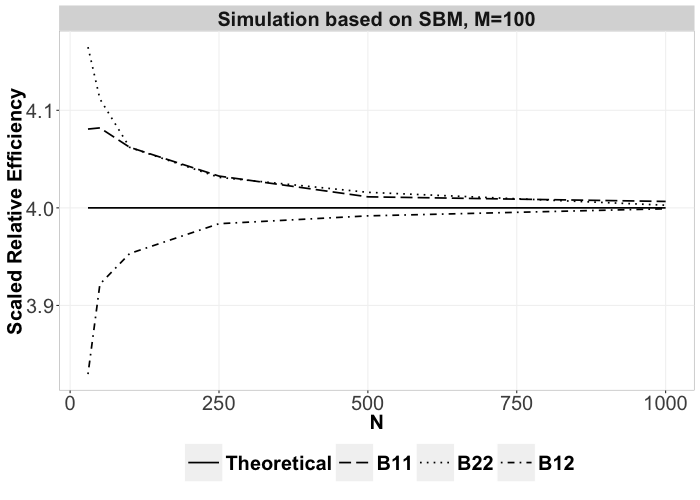
\includegraphics[width=1\textwidth]{RE.png}
	\caption{Scaled relative efficiency in average with different $N$ and fixed $M$ based on 1000 Monte Carlo replicates. Different types of dashed lines denote the simulated scaled RE associated with the edges we are averaging over. Solid line represents the theoretical value for scaled RE. Observe that $N \cdot \mathrm{RE}_{st}(\bar{A}, \hat{P})$ converges to $1/\rho_s + 1/\rho_t$ as expected.}
	\label{fig:RE}
\end{figure}

\begin{figure}[!htb]
\centering
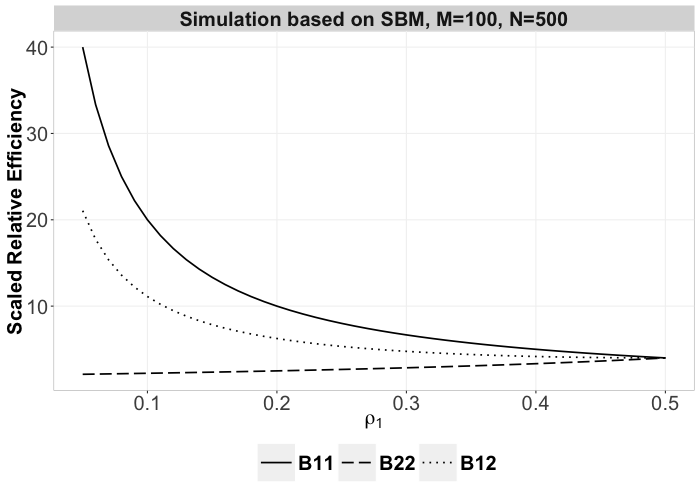
\includegraphics[width=1\textwidth]{Rho.png}
\caption{Simulated results for scaled RE, i.e. $N \cdot \mathrm{RE}_{st}(\bar{A}, \hat{P})$ with $N = 500$ and $M = 100$ of 1000 Monte Carlo replicates while changing $\rho_1$ from 0.1 to 0.9. Scaled relative efficiency in average with different $N$ and fixed $M$ based on 1000 Monte Carlo replicates. Different types of lines denote the simulated values associated with the edges we are averaging over. Notice that when $\rho_1 = 0.5$, the scaled RE has value $4.0$, which agrees with the result in Figure \ref{fig:RE} as expected.}
\label{fig:RErho}
\end{figure}

\subsection{CoRR Brain Graphs: Cross-Validation}
\begin{itemize}
\item In practice, the graphs may not perfectly follow an RDPG, or even not IEM. But we are still interested in the mean graph. To demonstrate that the $\hat{P}$ estimate is still valid in such cases, we examine three datasets, JHU, desikan and CPAC200, which are sets of 454 brain connectomes with different number of nodes generated from fMRI scans available at the Consortium for Reliability and Reproducibility (CoRR).
\item To compare $\bar{A}$ and $\hat{P}$ we perform a cross-validation study to examine the impact of the number of available graphs $M$.
\item Figure \ref{fig:realdata} demonstrates that our algorithm gives a better estimate $\hat{P}$ according to all three datasets. 
\item When $M$ is small, $\bar{A}$ has large variance which leads to large MSE. Meanwhile, $\hat{P}$ reduces the variance by taking advantages of the graph structure and outperforms $\bar{A}$ dramatically.
\item Moreover, Zhu and Ghodsi's algorithm and USVT algorithm both do a good job for selecting the dimension to embed.
\item Simulation with $P$ being the mean graph of the real data shows that $\hat{P}$ still does a good job when the low rank assumption is violated.
\end{itemize}

%\begin{figure}[!htb]
%\centering
%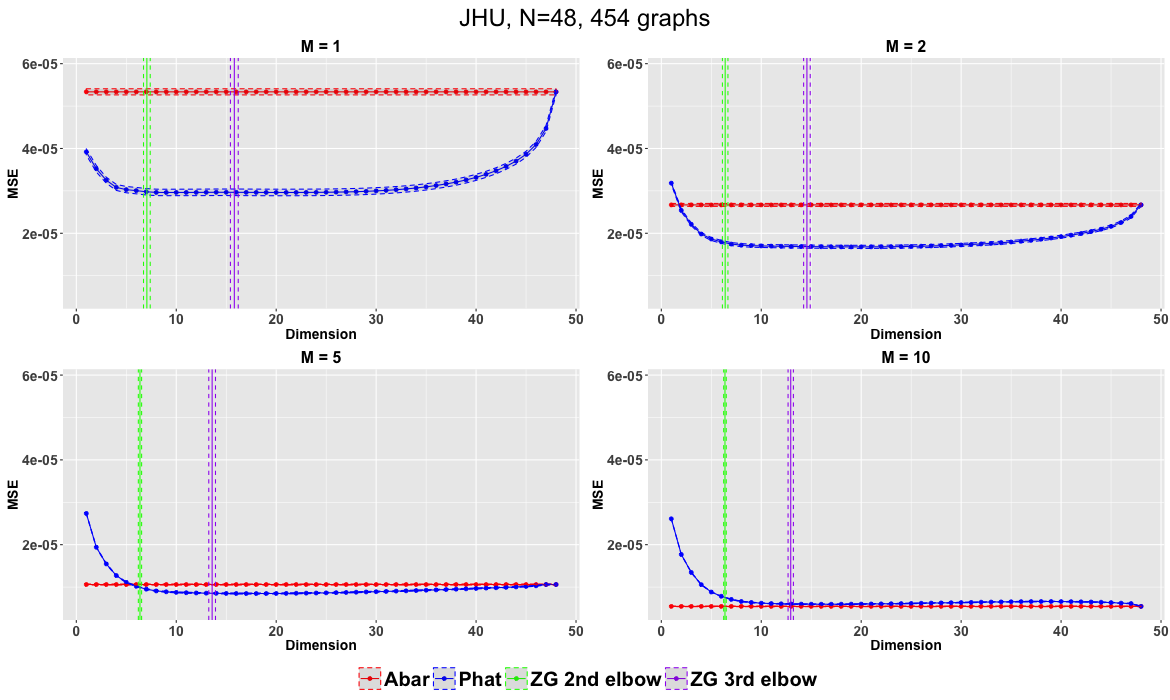
\includegraphics[width=1\textwidth]{JHU.png}
%\caption{Comparison of MSE between $\bar{A}$ (solid line) and $\hat{P}$ (dashed line) for JHU dataset while embedding the graphs into different dimensions with different size $M$ of the subsamples. The dimension chosen by the 3rd elbow of Zhu and Ghodsi is denoted in triangle, and chosen by USVT with threshold equals 0.7 is denoted in square. Vertical intervals represent the 95\% confidence interval. When $M$ is small, $\hat{P}$ outperforms $\bar{A}$ with a flexible range of the embedding dimension including what Zhu and Ghodsi selects.}
%\label{fig:JHU}
%\end{figure}
%
%\begin{figure}[!htb]
%\centering
%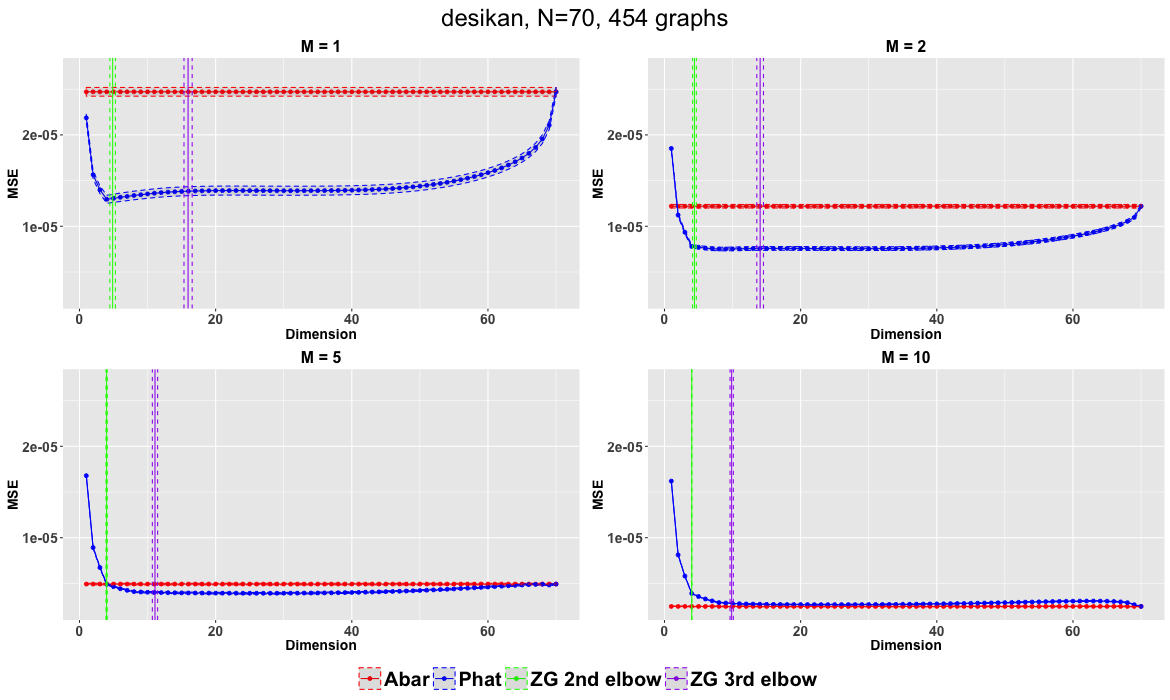
\includegraphics[width=1\textwidth]{desikan.png}
%\caption{Comparison of MSE between $\bar{A}$ (solid line) and $\hat{P}$ (dashed line) for desikan dataset while embedding the graphs into different dimensions with different size $M$ of the subsamples. The dimension chosen by the 3rd elbow of Zhu and Ghodsi is denoted in triangle, and chosen by USVT with threshold equals 0.7 is denoted in square.  Vertical intervals represent the 95\% confidence interval.  When $M$ is small, $\hat{P}$ outperforms $\bar{A}$ with a flexible range of the embedding dimension including what Zhu and Ghodsi selects.}
%\label{fig:desikan}
%\end{figure}
%
%\begin{figure}[!htb]
%\centering
%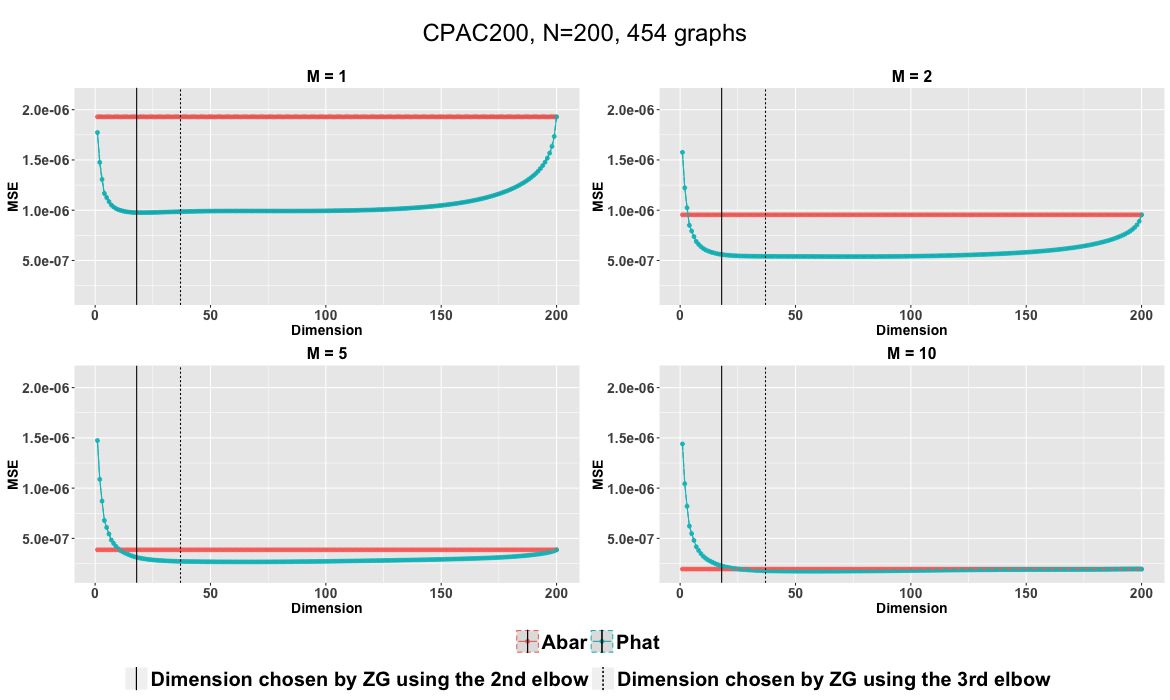
\includegraphics[width=1\textwidth]{CPAC200.png}
%\caption{Comparison of MSE between $\bar{A}$ (solid line) and $\hat{P}$ (dashed line) for CPAC200 dataset while embedding the graphs into different dimensions with different size $M$ of the subsamples. The dimension chosen by the 3rd elbow of Zhu and Ghodsi is denoted in triangle, and chosen by USVT with threshold equals 0.7 is denoted in square.  Vertical intervals represent the 95\% confidence interval.  When $M$ is small, $\hat{P}$ outperforms $\bar{A}$ with a flexible range of the embedding dimension including what Zhu and Ghodsi selects.}
%\label{fig:CPAC200}
%\end{figure}


\begin{figure}[!htb]
\centering
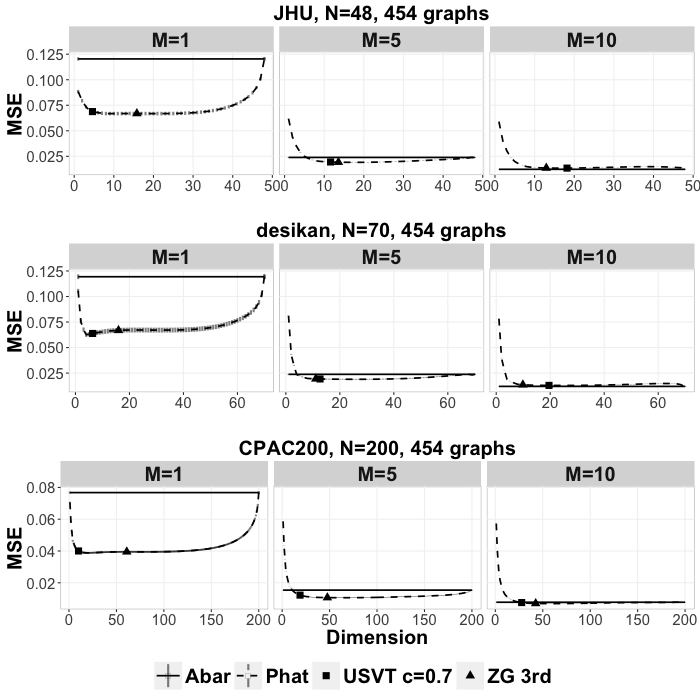
\includegraphics[width=1\textwidth]{realdata.png}
\caption{Comparison of MSE between $\bar{A}$ (solid line) and $\hat{P}$ (dashed line) for three dataset (JHU, desikan and CPAC200) while embedding the graphs into different dimensions with different size $M$ of the subsamples. The dimension chosen by the 3rd elbow of Zhu and Ghodsi is denoted in triangle (with largest 95\% confidence interval length to be $3.5$), and chosen by USVT with threshold equals 0.7 is denoted in square (with largest 95\% confidence interval length to be $0.7$).  Vertical intervals represent the 95\% confidence interval.  When $M$ is small, $\hat{P}$ outperforms $\bar{A}$ with a flexible range of the embedding dimension including what Zhu and Ghodsi selects.}
\label{fig:realdata}
\end{figure}




\begin{figure}[!htb]
\centering
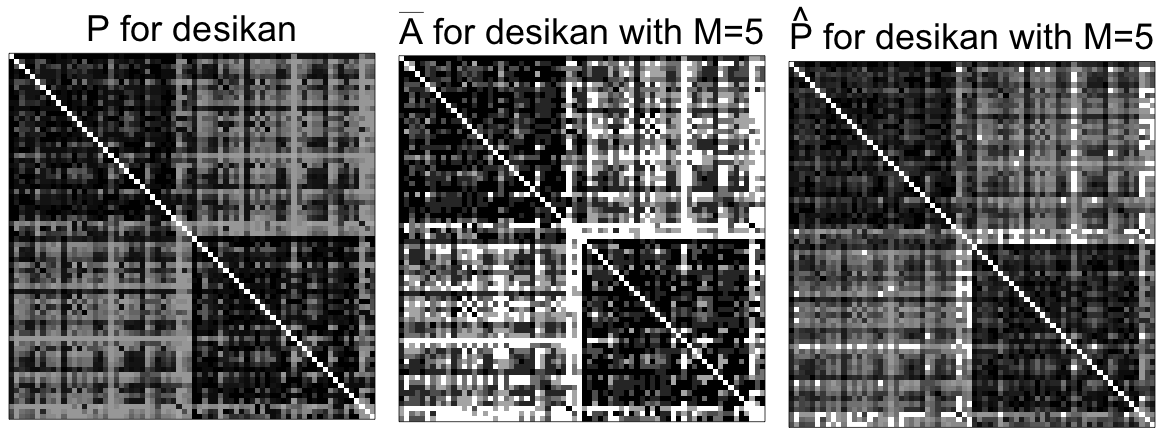
\includegraphics[width=1\textwidth]{Matrix_desikan_m5.png}
\caption{Comparison between the mean of 454 graphs $P$ and two estimates $\bar{A}$ and $\hat{P}$ derived from a sample of size $M=5$ from desikan dataset while embedding the graphs into dimension $d=11$ selected by the 3rd elbow of ZG method. From the figure, we can see that $\hat{P}$ is a better estimation of $P$ than $\bar{A}$.}
\label{fig:Matrix_desikan_m5}
\end{figure}

%\begin{figure}
%\centering
%\begin{subfigure}{.33\textwidth}
%  \centering
%  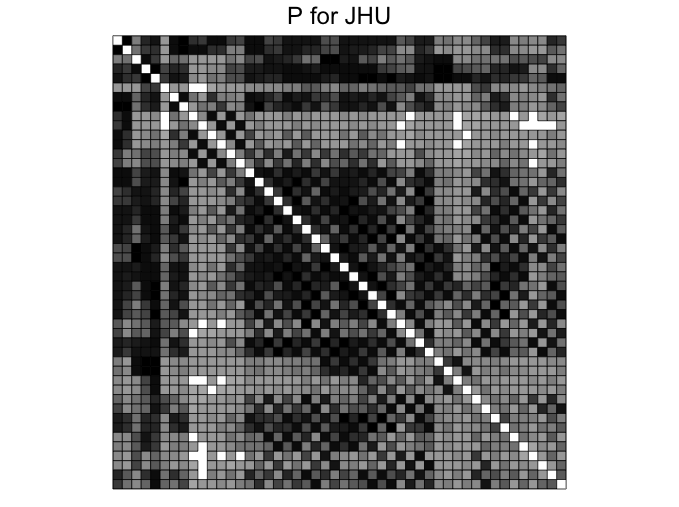
\includegraphics[width=1.2\linewidth]{P_JHU.png}
%\end{subfigure}%
%\begin{subfigure}{.33\textwidth}
%  \centering
%  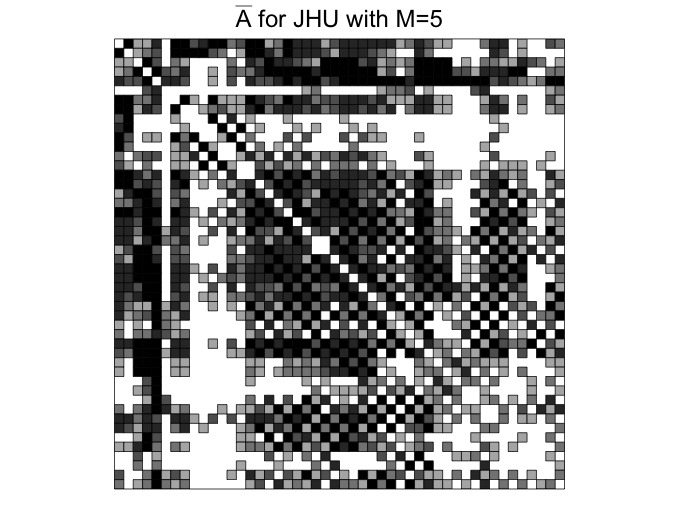
\includegraphics[width=1.2\linewidth]{Abar_JHU_m5.png}
%\end{subfigure}
%\begin{subfigure}{.33\textwidth}
%  \centering
%  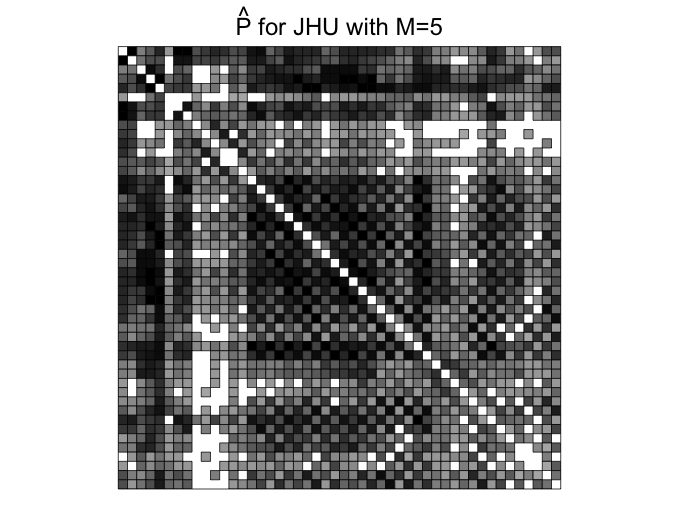
\includegraphics[width=1.2\linewidth]{Phat_JHU_m5.png}
%\end{subfigure}
%\caption{Comparison between the mean of 454 graphs $P$ and two estimates $\bar{A}$ and $\hat{P}$ derived from a sample of size $M=5$ from JHU dataset while embedding the graphs into dimension $d=15$ selected by the 3rd elbow of ZG method.}
%\label{fig:adj_JHU_m5}
%\end{figure}


\begin{figure}
\centering
\begin{subfigure}{.5\textwidth}
  \centering
  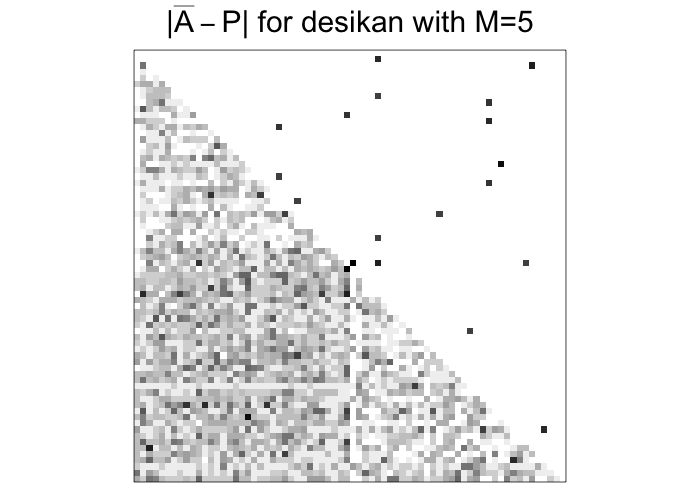
\includegraphics[width=1.2\linewidth]{Diff2_desikan_m5.png}
\end{subfigure}%
\begin{subfigure}{.5\textwidth}
  \centering
  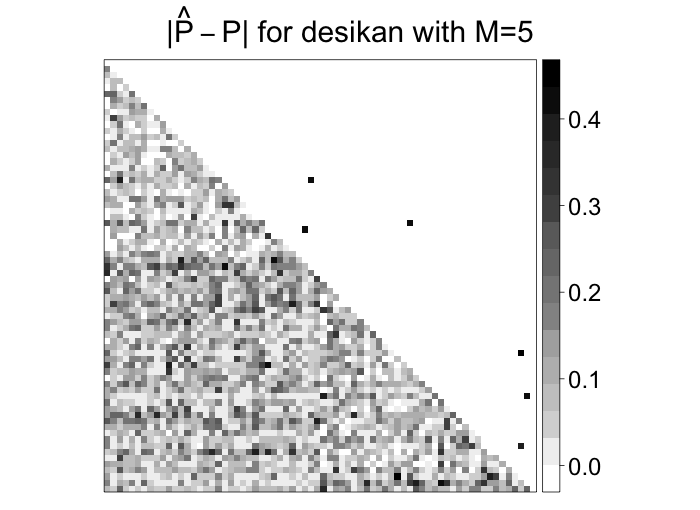
\includegraphics[width=1.2\linewidth]{Diff3_desikan_m5.png}
\end{subfigure}
\caption{Heat plot of the absolute estimation error $|\bar{A} - P|$ and $|\hat{P} - P|$ for a sample of size $M=5$ from desikan dataset while embedding the graphs into dimension $d=11$ selected by the 3rd elbow of ZG method. The lower triangular matrix shows the actual abstolute difference, while the upper triangular matrix only highlights the edges with absolute differences larger than $0.4$. The fact that 18 edges from $\bar{A}$ and 6 edges from $\hat{P}$ being highlighted shows the better performance of $\hat{P}$.}
\label{fig:Diff_desikan_m5}
\end{figure}



%\begin{figure}[!htb]
%\centering
%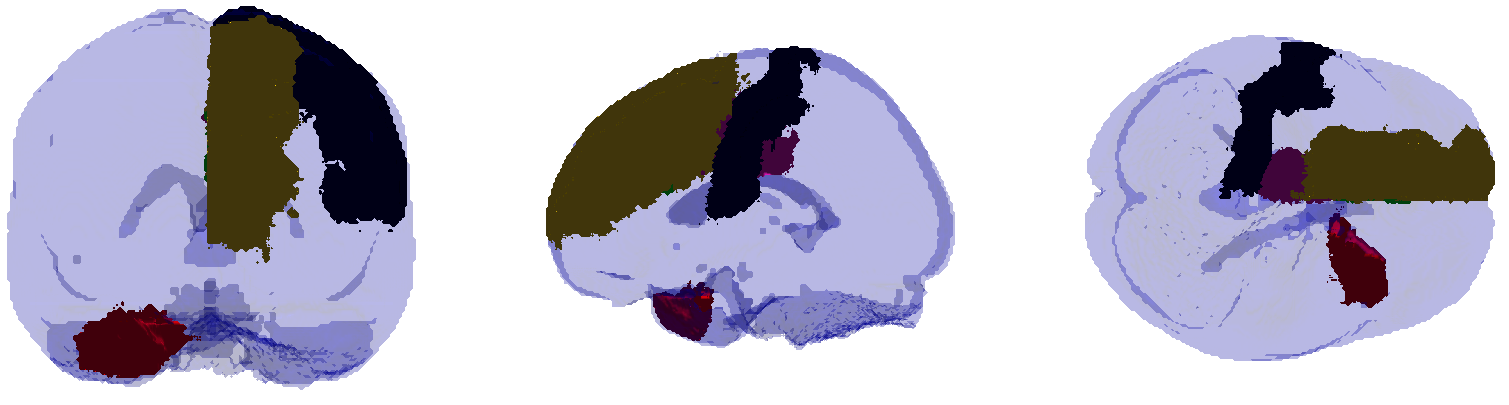
\includegraphics[width=1\textwidth]{Vertex_Diff_Phat_desikan.png}
%\caption{Top 5 regions of the brain (vertices in graphs) with largest absolute difference $|\hat{P} - P|$.}
%\label{fig:Vertex_Diff_Phat_desikan}
%\end{figure}
%
%\begin{figure}[!htb]
%\centering
%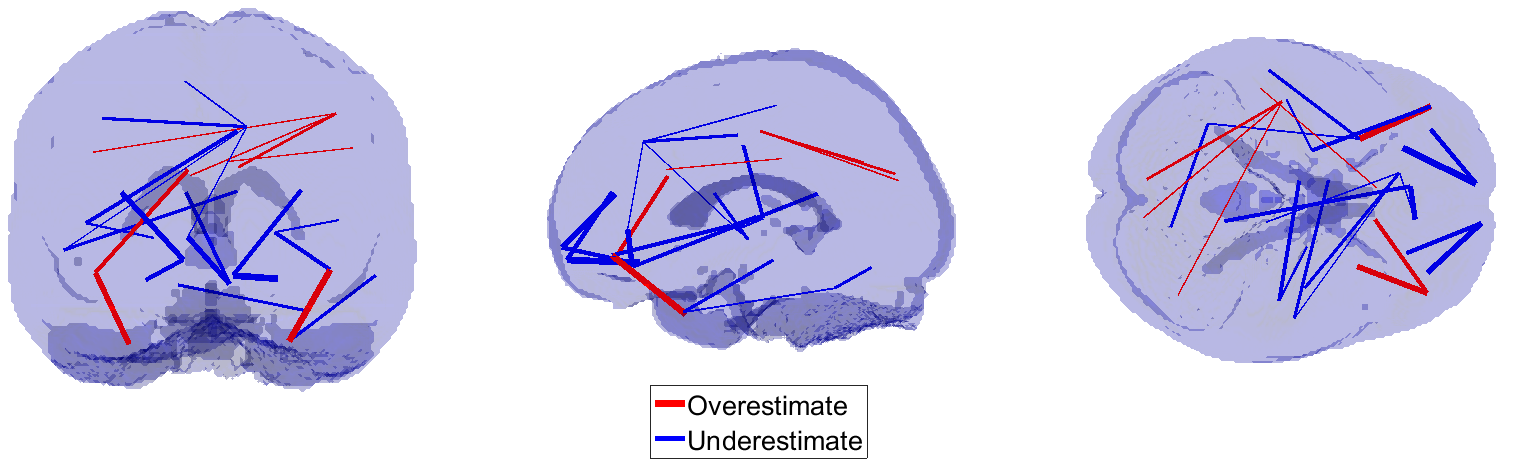
\includegraphics[width=1\textwidth]{Edge_Diff_Phat_desikan.png}
%\caption{Top 1\% (49) connections between regions (edges in graphs) with largest absolute difference $|\hat{P} - P|$.}
%\label{fig:Vertex_Diff_Phat_desikan}
%\end{figure}

\begin{figure}[!htb]
\centering
\includegraphics[width=1\textwidth]{Diff_between_desikan.png}
\caption{Top 5 regions of the brain (vertices in graphs) and top 50 connections between regions (edges in graphs) with largest difference $|\bar{A} - P| - |\hat{P} - P|$. Red indicates that $\hat{P}$ overestimate $P$ while blue means that $\hat{P}$ underestimate $P$. The edge width is determined by the estimation error. Connections with larger estimation error are represented by thicker lines. This figure shows the regions and connections of the brain where $\hat{P}$ outperforms $\bar{A}$ mostly for estimate $P$.}
\label{fig:Diff_between_desikan}
\end{figure}




\subsection{Simulation under the Full Rank Independent Edge Model}
\begin{itemize}
\item While the theory we have is based on the low rank assumption, $\hat{P}$ sometimes wins the bias-variance tradeoff even when the graphs have full rank structure. To illustrate this point, instead of the low rank SBM, we run simulations under the full rank independent edge model with the probability matrix $P$ to be the sample mean of the 454 graphs in the desikan dataset.
\item Figure \ref{fig:sim_desikan} compare the MSE between $\bar{A}$ (solid line) and $\hat{P}$ (dashed line) for simulated data based on the full rank probability matrix $P$ as the sample mean in desikan dataset while embedding the graphs into different dimensions with different size $M$ of the subsamples. Vertical intervals represent the 95\% confidence interval. When $M$ is small, $\hat{P}$ outperforms $\bar{A}$ with a flexible range of the embedding dimension including what Zhu and Ghodsi selects.
\end{itemize}

\begin{figure}[!htb]
\centering
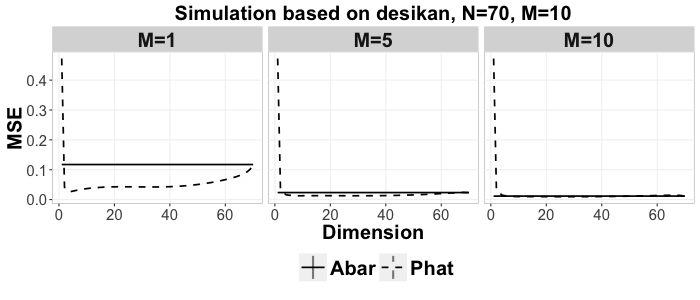
\includegraphics[width=1\textwidth]{sim_desikan.png}
\caption{Comparison of MSE between $\bar{A}$ (solid line) and $\hat{P}$ (dashed line) for simulated data based on the full rank probability matrix $P$ as the sample mean in desikan dataset while embedding the graphs into different dimensions with different size $M$ of the subsamples. Vertical intervals represent the 95\% confidence interval. When $M$ is small, $\hat{P}$ outperforms $\bar{A}$ with a flexible range of the embedding dimension including what Zhu and Ghodsi selects.}
\label{fig:sim_desikan}
\end{figure}



\section{Discussion}

\subsection{Summary}
\begin{itemize}
\item In this paper, we propose a better way to estimate the mean of a collection of graphs by taking advantage of the low rank structure of the graphs.
\end{itemize}

\subsection{Future Work}
\begin{itemize}
\item Generally the observations we have are always contaminated in practice. In this case, improved robust estimator based on the low rank structure of the graphs is preferred.
\item Estimating the rank of the graph structure accurately will certainly help improve the results.
\item In this paper, we are using Scheinerman's method with 1 iteration for diagonal augmentation.
\end{itemize}






\section{Methods}

\subsection{Choosing Dimension}
\label{section:dim_select}
\begin{itemize}
\item Often in dimensionality reduction techniques, the choice for dimension, d, relies on visually analyzing a plot of the ordered eigenvalues, looking for a ``gap'' or ``elbow'' in the scree-plot.
\item USVT is a simple estimation procedure that works for any matrix that has ``a little bit of structure''.
\end{itemize}

\subsection{Graph Diagonal Augmentation}
\label{section:diag_aug}
\begin{itemize}
\item The graphs examined in this work are hollow, in that there are no self-loops and thus the diagonal entries of the adjacency matrix are 0. This leads to a bias in the calculation of the eigenvectors.
\item We minimize this bias by using an iterative method developed by Scheinerman and Tucker.
\end{itemize}

\subsection{Source Code}

\subsection{Dataset Description}
\begin{itemize}
\item The original dataset is from the Emotion and Creativity One Year Retest Dataset provided by Qiu, Zhang and Wei from Southwest University. It is comprised of 235 subjects, all of whom were college students. Each subject underwent two sessions of anatomical, resting state DTI scans, spaced one year apart. Due to the incomplete data, the true number of scans is 454.
\item When deriving MR connectomes, the NeuroData team parcellate the brain into groups of nodes as defined by anatomical atlases. The atlases are defined either physiologically or structurally by neuroanatomists (Desikan and JHU), or are generated using a segmentation algorithm looking for certain features or groupings (CPAC200).
\item The graphs we are using are processed by NeuroData team from DTI data of the original dataset generated with different atlases (desikan, JHU and CPAC200), each containing different region/node definitions.
\item The graphs are undirected, unweighted and with no self-loops. An edge exists between two regions when there is at least one white-matter tract connecting the corresponding two parts of the brain.
\end{itemize}

\subsection{Outline for the Proof of the Theorems}



\bibliography{Bib}{}
\bibliographystyle{plain}


\end{document}